% BACKGROUND & RELATED WORK
%
% !TEX root = ../thesis-main.tex
%
\chapter{Background and related work}
\label{chap:background}

%\cleanchapterquote{You can’t do better design with a computer, but you can speed up your work enormously.}{Wim Crouwel}{(Graphic designer and typographer)}

\blindtext 

\blindtext


\section{Computer-Assisted Pronunciation Tutoring} %TODO Teaching,Training?
	\subsection{Pronunciation in foreign language education}
	\subsection{Computer-based and intelligent tutoring systems}
	\subsection{Survey of existing CAPT systems}
	
	

\section{Towards CAPT for French learners of German}

	\subsection{Phonetic and phonological comparison}
		\subsubsection{Segments}
		\subsubsection{Prosody}
		\subsubsection{Other factors}
		
	\subsection{Targeting lexical stress errors}
		\blindtext
		\begin{center}
		\begin{figure}[htb]
			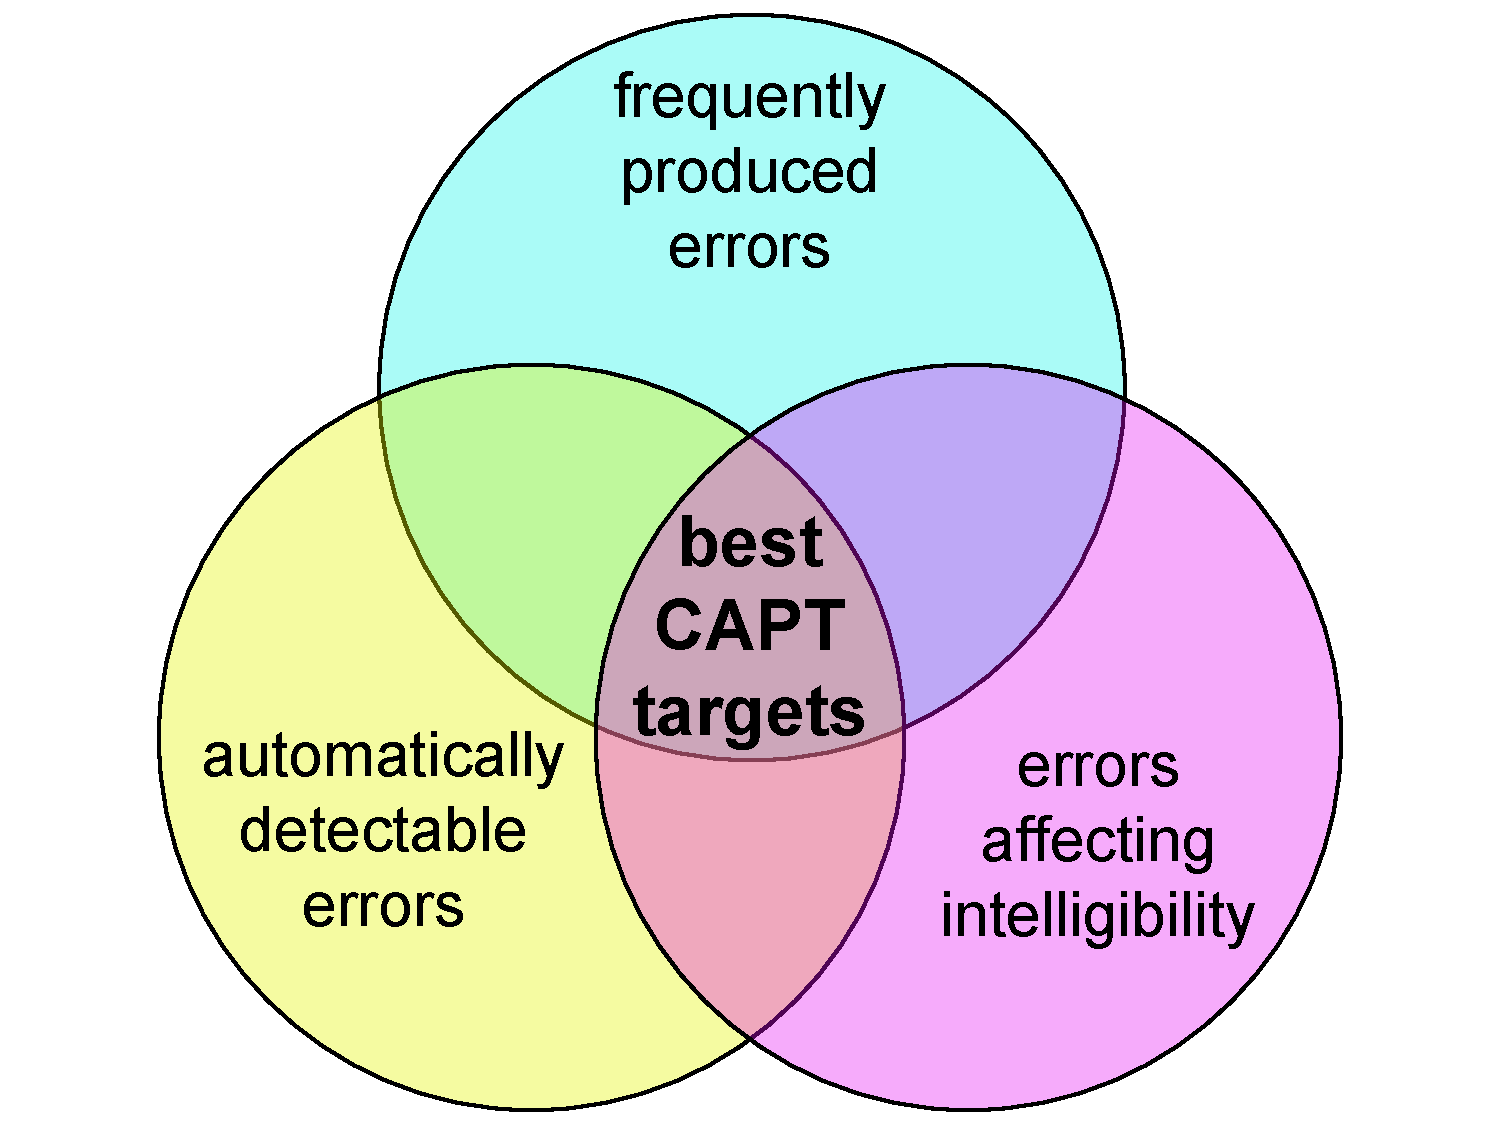
\includegraphics[width=.7\textwidth]{../img/error-venn}
			\caption{Criteria for selecting errors to target in a CAPT system.}
			\label{fig:errors}
		\end{figure}
		\end{center}
		\subsubsection{Frequency of production}
		\subsubsection{Impact on intelligibility}
		\subsubsection{Feasibility of automatic detection}
		
\section{Summary}